\documentclass{report}
\usepackage{homework}
\solstrue

\renewcommand{\hmwkTitle}{Homework 8}
\usepackage{booktabs}
\usepackage{mathtools}

\begin{document}
\mktitle

\begin{problem}

When a BGP router receives an advertised path from a neighbor, it can choose add its own AS number to the received path and then advertise that new path to of its neighbors. But for some of the paths received, they are not included in the advertised new path to some or all the neighbors. Please find out at least two reasons why this is the case.

\begin{answer}{40em}
    \begin{enumerate}
        \item An ISP may not want to route other ISPs' traffic through itself. So, it will not include
            itself in the advertised path.
        \item It will not include itself in the advertised path if including itself forms a loop; i.e.
            if the path an ISP receives already includes the ISP, it will not include itself again.
    \end{enumerate}
\end{answer}
\end{problem}

\newpage
\begin{problem}
We learned about network address translation (NAT) in chapter 4. For IP packets with TCP or UDP segments as payload, NAT translates both IP address in the IP header and port number in the transport layer (i.e., TCP or UDP) header. In chapter 5, we learned ICMP protocol as another possible kind of payload inside IP packets. Despite the lack of dedicated ``port number'' field in the ICMP header, the majority of NAT-capable routers can properly handle ICMP messages when they travel between the private network and the public network. This allows diagnostic programs that use ICMP, such as \texttt{ping} and \texttt{traceroute}, to function inside a private network with NAT. Here we explore the latter case and see why it is true.

Let's suppose that a private subnet with the address range \texttt{192.168.10.0/24} is connected to the Internet using a NAT-capable router. The NAT router has a single public address \texttt{131.179.11.30}, which it uses for all communication with
hosts that are not part of the private network. A host inside the private network with IP address \texttt{192.168.10.5} is running \texttt{traceroute 8.8.8.8}. The \texttt{traceroute} program sends UDP segments from \texttt{192.168.10.5:12345} to \texttt{8.8.8.8:39427}. The translation table inside the router contains the following entries:

\begin{table}[H]
  \caption{NAT Translation Table}
  \label{tbl:nat}
  \centering \smallskip
  \begin{tabular*}{0.7\textwidth}{c c}
    \toprule
    \texttt{IP:port} within private network &  \texttt{IP:port} outside private network \\
    \midrule
    \texttt{192.168.10.5:5000} & \texttt{131.179.11.30:8000} \\
    \midrule
    \texttt{192.168.10.2:12345} & \texttt{131.179.11.30:8001} \\
    \midrule
    \texttt{192.168.10.5:12345} & \texttt{131.179.11.30:8002} \\
    \midrule
    $\ldots$ & $\ldots$ \\
    \bottomrule
  \end{tabular*}
\end{table}

Suppose that one of the IP packets generated by the above \texttt{traceroute} program arrives at router \texttt{76.167.29.184} and the TTL field in the IP header is 0. We use ``Packet A'' to refer to this packet as received by \texttt{76.167.29.184} below.

\begin{enumerate}
\item What are the source and destination addresses (IP and port) of Packet A?
\item Upon receiving Packet A, the router \texttt{76.167.29.184} drops it and generates an ICMP message (referred to as ``Message B'' below). What are the values of type and code fields within the ICMP message? What are the source and destination IP addresses of Message B? (Hint: refer to the lecture slides on traceroute)
\item According to RFC 792, Message B (generated by router) is sent back to the source IP address of packet A. It also includes the IP header and the first 64 bit of IP payload (in this case, the \textbf{UDP header}) of packet A. The format of ICMP message is given below. When this message arrives at the NAT router, what are the actions that the NAT router needs to take so that Message B will arrive at host \texttt{192.168.10.5}? (Hint: Try to think if the NAT router can find out the type of the packet containing message B, and find out the address information from inside, given the message content below.)
\begin{verbatim}
    Bits
    0                   1                   2                   3
    0 1 2 3 4 5 6 7 8 9 0 1 2 3 4 5 6 7 8 9 0 1 2 3 4 5 6 7 8 9 0 1
   +-+-+-+-+-+-+-+-+-+-+-+-+-+-+-+-+-+-+-+-+-+-+-+-+-+-+-+-+-+-+-+-+
   |     Type      |     Code      |          Checksum             |
   +-+-+-+-+-+-+-+-+-+-+-+-+-+-+-+-+-+-+-+-+-+-+-+-+-+-+-+-+-+-+-+-+
   |                             unused                            |
   +-+-+-+-+-+-+-+-+-+-+-+-+-+-+-+-+-+-+-+-+-+-+-+-+-+-+-+-+-+-+-+-+
   |      Internet Header + 64 bits of Original Data Datagram      |
   +-+-+-+-+-+-+-+-+-+-+-+-+-+-+-+-+-+-+-+-+-+-+-+-+-+-+-+-+-+-+-+-+
\end{verbatim}
\end{enumerate}

\begin{answer}{40em}
    \begin{enumerate}
        \item The source and destination addresses of Packet A are \texttt{131.179.11.30.8002} and 
            \texttt{8.8.8.8:39427} respectively
        \item The value of type is 11 and the value of code is 0. The source and destination IP addresses
            of Message B are \texttt{76.167.29.184} and \texttt{131.179.11.30} respectively.
        \item The NAT will demux the IP datagram to ICMP and read the header. This header will
            contain the destination port so that the NAT can translate from public to private IP.
    \end{enumerate}
\end{answer}
\end{problem}

\newpage
\begin{problem}

Answer the following questions about CSMA/CD.

\begin{enumerate}
    \item In CSMA/CD, after the fifth collision, what is the probability that a node chooses backoff interval $K = 4$?
    \item When choosing backoff window, CSMA/CD starts from a small range for $K$ and exponentially increase it if more collision happen. What is the reasoning behind this design? (Hint: Read textbook section 6.3.2)
\end{enumerate}

\begin{answer}{40em}
    \begin{enumerate}
        \item $n = 5 \implies \{0, \ldots, 2^{n = 5} - 1 = 31\}$. Then $\frac{1}{31} = 0.0322$.
        \item We use exponential backoff because we want to decrease the probability of another collision
            as the number of collisions/nodes arriving increases; i.e. we want to minimize the number
            of collisions as quickly as possible.
    \end{enumerate}
\end{answer}

\end{problem}

\newpage
\begin{problem}
In this problem, you will derive the efficiency of a CSMA/CD like multiple access protocol.
In this protocol, time is slotted and all adapters are synchronized to the slots.
Unlike slotted ALOHA, however, the length of a slot (in seconds) is much less than a frame time (the time to transmit a frame).
Let $S$ be the length of a slot.
Suppose all frames are of constant length $L = kRS$, where $R$ is the transmission rate of the channel and $k$ is a large integer.
Suppose there are $N$ nodes, each with an infinite number of frames to send.
We also assume that $d_{prop} < S$, so that all nodes can detect a collision before the end of a slot time.
The protocol is as follows:

\begin{itemize}
\item If no node has possession of the channel for a given slot, all nodes contend for the channel; in particular, each node transmits in the slot with probability $p$. If exactly one node transmits in the slot, that node takes possession of the channel for the subsequent $k-1$ slots and transmits its frame.
\item If some node has possession of the channel, all other nodes refrain from transmitting until the node that possesses the channel has finished transmitting its frame. Once this node has transmitted its frame, all nodes contend for the channel.
\end{itemize}

Note that the channel alternates between two states: the productive state, which lasts exactly $k$ slots, and the non-productive state, which lasts for a random number of slots.
The channel efficiency is defined as the ratio of $k/(k+x)$, where $x$ is the expected number of consecutive non-productive slots.

\begin{enumerate}
\item For fixed $N$ and $p$, determine the efficiency of this protocol.
\item For fixed $N$, determine the $p$ that maximizes the efficiency.
\end{enumerate}

  \begin{answer}{60em}
      \begin{enumerate}
          \item We have that the probability of failure is $\left(1 - Np(1 - p)^{N - 1}\right)^{m - 1}(Np(1 - p)^{N - 1})$
              which is a geometric distribution $\implies$ $x = \frac{1 - Np(1 - p)^{N - 1}}{Np(1 - p)^{N - 1}}$. Then,
              we get that the efficiency of this protocol is 
              \[\frac{k}{k + \frac{1 - Np(1 - p)^{N - 1}}{Np(1 - p)^{N - 1}}}\]
          \item To determine the $p$ that maximizes efficiency, we do
              \[\frac{\partial}{\partial p} \left(Np(1 - p)^{N - 1}\right) = \frac{N(1 - p)^N(Np - 1)}{(p - 1)^2}\]
              solving for the maximum, we get that $p = \frac{1}{N}$.
      \end{enumerate}
  \end{answer}

\end{problem}

\begin{problem}

Consider the network shown in the following figure. The three subnets are interconnected by two routers R1 and R2. Within each subnet, there is an Ethernet switch (S1, S2 and S3 in the figure).

\begin{center}
    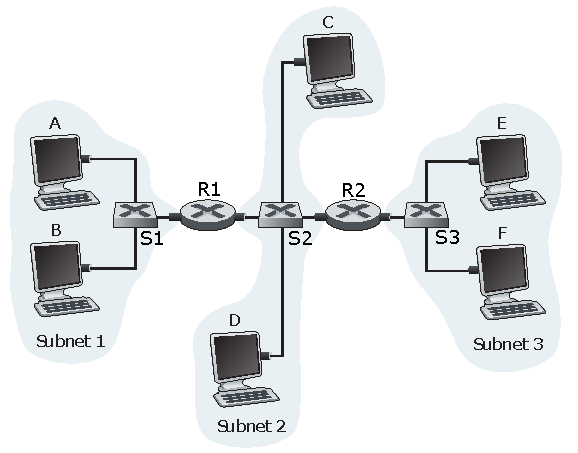
\includegraphics[width=0.5\linewidth]{figures/hw8-rs.pdf}
\end{center}

\begin{enumerate}
    \item Consider sending an IP datagram from Host E to Host F. Will Host E ask router R2 to help forward the datagram? Why? In the Ethernet frame containing the IP datagram, what are the source and destination IP and MAC addresses?
    \item Suppose Host E would like to send an IP datagram to Host B, and assume that E’s  ARP cache does not contain B’s MAC address. Will E perform an ARP  query to find B’s MAC address? Why? In the Ethernet frame (containing  the IP datagram destined to B) that is delivered to router R2, what are the source and destination IP and MAC addresses?

\end{enumerate}

\begin{answer}{30em}
    \begin{enumerate}
        \item No, Host E will not ask R2 to help forward the datagram since F belongs to the same
            subnet. The Ethernet frame will have a source IP and MAC address of E and a destination
            IP and MAC address F. This assumes that the ARP cache in the host is non-empty.
        \item No, because Host E and B are in different subnets. The Ethernet frame will have a
            source IP and MAC address E and a destination IP address R2 and MAC address B.
    \end{enumerate}
\end{answer}
\end{problem}


\end{document}
